\usetikzlibrary{calc,shapes.geometric}
\begin{tabular}{@{}c@{\hspace{6mm}}c@{}}
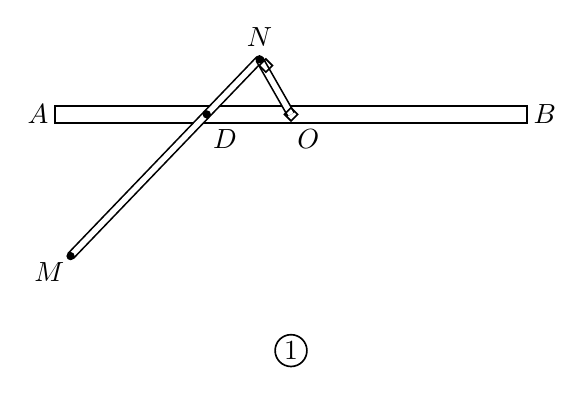
\begin{tikzpicture}[x=1cm,y=1cm,line width=.6pt,>=stealth,font=\normalsize]
\draw (0,-0.11) rectangle (6,0.11);
\draw[double distance=2pt] (0.2,-1.8) -- (2.6,0.7);
\draw[double distance=2pt] (3.0,0) -- (2.6,0.7);
\node[diamond,draw,minimum size=5pt,inner sep=0pt] at (2.68,0.62) {};
\node[diamond,draw,minimum size=5pt,inner sep=0pt] at (3.0,0) {};
\fill (0.2,-1.8) circle[radius=1.5pt];
\fill (1.93,0) circle[radius=1.5pt];
\fill (2.6,0.7) circle[radius=1.5pt];
\node[left,inner sep=0pt,xshift=-2pt] at (0,0) {$A$};
\node[right,inner sep=0pt,xshift=2pt] at (6,0) {$B$};
\node[below left,inner sep=0pt,xshift=-2pt,yshift=-2pt] at (0.2,-1.8) {$M$};
\node[below right,inner sep=0pt,xshift=2pt,yshift=-2pt] at (1.93,-0.11) {$D$};
\node[below right,inner sep=0pt,xshift=2pt,yshift=-2pt] at (3.0,-0.11) {$O$};
\node[above,inner sep=0pt,yshift=2pt] at (2.6,0.78) {$N$};
\node[draw,circle,inner sep=1.2pt] at (3,-3.0) {1};
\end{tikzpicture}
&
\begin{tikzpicture}[x=1cm,y=1cm,line width=.6pt,>=stealth,font=\normalsize]
\draw[->] (-4.0,0) -- (2.2,0) node[right,inner sep=0pt,xshift=2pt] {$x$};
\draw[->] (0,-2.2) -- (0,2.2) node[above,inner sep=0pt,yshift=2pt] {$y$};
\draw (-3.0,-1.8) -- (-1.2,0) -- (-0.6,0.6) -- (0,0);
\node[below left,inner sep=0pt,xshift=-2pt,yshift=-2pt] at (-3.0,-1.8) {$M$};
\node[below right,inner sep=0pt,xshift=2pt,yshift=-2pt] at (-1.2,0) {$D$};
\node[below right,inner sep=0pt,xshift=2pt,yshift=-2pt] at (0,0) {$O$};
\node[above left,inner sep=0pt,xshift=-2pt,yshift=2pt] at (-0.6,0.6) {$N$};
\node[draw,circle,inner sep=1.2pt] at (-0.9,-3.0) {2};
\end{tikzpicture}
\end{tabular}
